% *********************************************************************
% © 2021–2024 Jeremy Sylvestre
%
% Permission is granted to copy, distribute and/or modify this document
% under the terms of the GNU Free Documentation License, Version 1.3 or
% any later version published by the Free Software Foundation; with no
% Invariant Sections, no Front-Cover Texts, and no Back-Cover Texts. A
% copy of the license is included in the appendix entitled “GNU Free
% Documentation License” that appears in the output document of this
% PreTeXt source code. All trademarks™ are the registered® marks of
% their respective owners.
%
% *********************************************************************

\newcommand*{\xmin}{0}
\newcommand*{\xmax}{10}
\newcommand*{\ymin}{0}
\newcommand*{\ymax}{6}

%
% DE is y' = r (M - y) y
%
% We are using r = 1 and M = 4
%
% Solutions curves are
%   y = 4 A e^{4t} / (1 + A e^{4t})
% where
%   A = y0 / (4 - y0)
% but for A≠0 we can rearrange to
%   y = 4 / (B e^{-4t} + 1)
% where
%   B = 1/A = (4 - y0) / y0
% BUT
% we have h.scaled solutions by a factor of 10

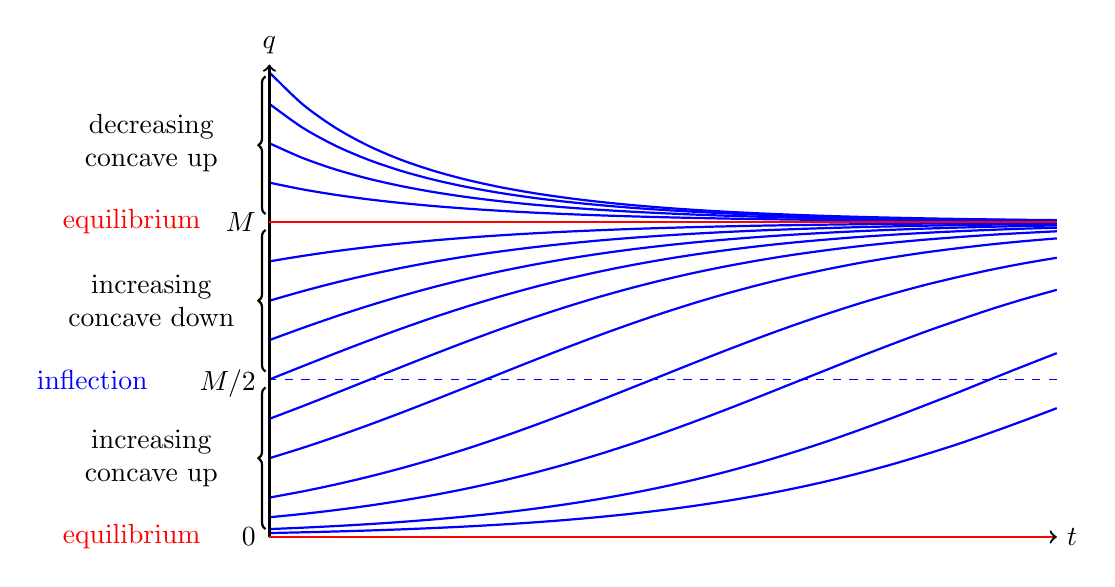
\begin{tikzpicture}
[
	closedpt/.style={circle,draw,fill,inner sep=0pt,minimum size=4pt},
	openpt/.style={circle,draw,inner sep=0pt,minimum size=4pt}
]

	\draw[dashed,blue] (\xmax,2) -- (\xmin,2);
	\node[left,xshift=-0.05cm,yshift=-0.05cm] at (0,2) {$M/2$};
	\node[blue,xshift=-2.25cm] at (0,2) {inflection};

	\draw[thick, decorate, decoration = {brace}, xshift=-0.05cm] (0,4.1) -- (0,5.85);
	\node[align=center,xshift=-1.5cm] at (0,5) {decreasing \\ concave up};

	\draw[thick, decorate, decoration = {brace}, xshift=-0.05cm] (0,2.1) -- (0,3.9);
	\node[align=center,xshift=-1.5cm] at (0,3) {increasing \\ concave down};

	\draw[thick, decorate, decoration = {brace}, xshift=-0.05cm] (0,0.1) -- (0,1.9);
	\node[align=center,xshift=-1.5cm] at (0,1) {increasing \\ concave up};

	\foreach \q in {0.05,0.1,0.25,0.5,1,1.5,2,2.5,3,3.5,4.5,5,5.5,5.9} {
		\draw[thick,blue,smooth,domain=0:\xmax] plot (\x, { 4 / (1 + (4 - \q) * exp(-4*\x/10) / \q) });
	}

	% axes
	\draw[->,thick] (\xmin,0) -- (\xmax,0) node[right] {$t$};
	\draw[->,thick] (0,\ymin) -- (0,\ymax) node[above] {$q$};

	\foreach \q in {0,4} {
		\node[red,xshift=-1.75cm] at (0,\q) {equilibrium};
	}
	\draw[red,thick] (9.95,0) -- (\xmin,0);
	\draw[red,thick] (\xmax,4) -- (\xmin,4);
	\node[left,xshift=-0.05cm] at (0,0) {$0$};
	\node[left,xshift=-0.05cm] at (0,4) {$M$};

\end{tikzpicture}
